\documentclass[tikz,crop]{standalone}

% Part of the preamble, for TikZ figures.
% This is used in both the main document and in the subfigures.
% One exception is minted: since the path depends on the file, it is not set.
\usepackage{tikz}
\usepackage{xcolor}
\usepackage{pgfplots}

\pgfplotsset{compat=1.18}
\usepgfplotslibrary{statistics}

\usetikzlibrary{shapes,arrows,positioning,backgrounds,calc,intersections,calc}

\definecolor{ugent-re}{RGB}{220, 78, 40}        % vermilion			/ vermiljoen
\definecolor{ugent-we}{RGB}{45, 140, 168}       % no match
\definecolor{ugent-ge}{RGB}{232, 94, 113}       % rose				/ bleekrood
\definecolor{ugent-ea}{RGB}{111, 113, 185}      % distant blue		/ verblauw
\definecolor{ugent-pp}{RGB}{251, 126, 58}       % deep orange		/ dieporanje
\definecolor{ugent-ps}{RGB}{113, 168, 96}       % yellow green		/ geelgroen

\tikzstyle{python}=[fill=ugent-ps!50!white]
\tikzstyle{java}=[fill=ugent-we!50!white]
\tikzstyle{haskell}=[fill=ugent-ea!50!white]
\tikzstyle{js}=[fill=ugent-pp!50!white]
\tikzstyle{c}=[fill=ugent-re!50!white]

\newlength{\block}
\setlength{\block}{0.75cm}

\tikzstyle{a}=[anchor=north west]
\tikzstyle{box}=[a,draw,rectangle]
\tikzstyle{node}=[a,draw,minimum height=0.5cm,align=center,fill=white,text depth=.25ex]
\tikzstyle{document}=[node,tape,tape bend top=none]
\tikzstyle{cont}=[box,minimum height=1\block,minimum width=1\block]
\tikzstyle{arrow}=[draw, -latex]
\tikzstyle{inner}=[box,draw=gray]

% Blue box style
\tikzstyle{bluebox}=[draw=ugent-we,java]
\tikzstyle{redbox}=[draw=ugent-re,c]
\tikzstyle{greenbox}=[draw=ugent-ps,python]

% Some things specific to TESTed imagery.
\tikzstyle{tc}=[box,draw=ugent-ps]
\tikzstyle{comp}=[box,draw=ugent-re,fill=ugent-re,fill opacity=0.05]
\tikzstyle{exec}=[box,draw=ugent-we,fill=ugent-we,fill opacity=0.10]

% Stuff from tested-engine/concept.tex
\tikzstyle{process}=[node,rectangle]
\tikzstyle{terminator}=[node,rectangle,rounded corners=0.5cm]
\tikzstyle{io}=[node,trapezium,trapezium left angle=70,trapezium right angle=-70,minimum width=2.5cm,trapezium stretches=true]
\tikzstyle{small}=[font=\footnotesize,color=darkgray]
\tikzstyle{submission}=[document,align=right,minimum width=3cm,minimum height=1cm,text depth=0.5cm,inner sep=0.5mm,font=\scriptsize]

% Stuff from chatper3/flow.tex
\tikzstyle{height}=[minimum height=0.75\block]
\tikzstyle{contt}=[cont,minimum height=0.75\block]
\tikzstyle{compop}=[comp,text opacity=1]
\tikzstyle{execop}=[exec,text opacity=1]

\tikzstyle{hnode}=[draw,anchor=center,minimum height=\block,text depth=.25ex,align=center]
\tikzstyle{executable}=[hnode,ultra thick,fill=gray!10]
\tikzstyle{inner-exec}=[node,anchor=center,minimum width=3.25\block,densely dotted,font=\footnotesize,fill=none]
\tikzstyle{stmt}=[node,anchor=center,fill=gray!30,minimum width=4.5\block,font=\footnotesize]
\tikzstyle{fieldset}=[minimum height=\block,fill=white,text depth=.5ex,fill=white]

% Minted environments for use in Tikz
\newminted[tikzjava]{java}{autogobble,linenos=false,fontsize=\tiny,stripall}
\newminted[tikzpython]{python}{autogobble,linenos=false,fontsize=\tiny,stripall}
\newminted[tikztext]{text}{autogobble,linenos=false,fontsize=\tiny,stripall}


\begin{document}

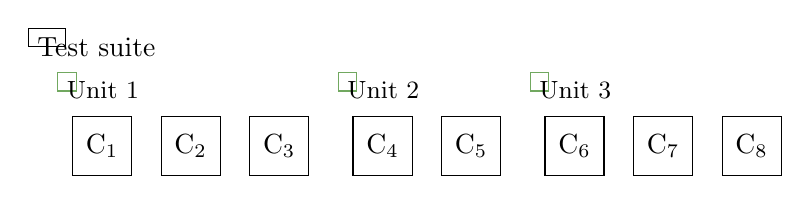
\begin{tikzpicture}[x=0.75cm,y=0.75cm]
%    \draw[step=1,gray!10,thin] (0,0) grid (14,-20);

    \node[box,minimum height=3\unit, minimum width=13.5\unit] at (0,0) (ts1) {};
    \node[below right] at (ts1.north west) {Test suite};

    \node[cont] at (0.75, -1.5) (ts1c1) {C\textsubscript{1}};
    \node[cont] at (2.25, -1.5) (ts1c2) {C\textsubscript{2}};
    \node[cont] at (3.75, -1.5) (ts1c3) {C\textsubscript{3}};
    \node[tc,minimum height=2\unit,minimum width=4.5\unit] at (0.5,-0.75) (tc1) {};
    \node[below right] at (tc1.north west) {\small Unit 1};

    \node[cont] at (5.50, -1.5) (ts1c4) {C\textsubscript{4}};
    \node[cont] at (7.00, -1.5) (ts1c5) {C\textsubscript{5}};
    \node[tc,minimum height=2\unit,minimum width=3\unit] at (5.25,-0.75) (tc2) {};
    \node[below right] at (tc2.north west) {\small Unit 2};

    \node[cont] at (8.75, -1.5) (ts1c6) {C\textsubscript{6}};
    \node[cont] at (10.25, -1.5) (ts1c7) {C\textsubscript{7}};
    \node[cont] at (11.75, -1.5) (ts1c8) {C\textsubscript{8}};
    \node[tc,minimum height=2\unit,minimum width=4.5\unit] at (8.5,-0.75) (tc3) {};
    \node[below right] at (tc3.north west) {\small Unit 3};
\end{tikzpicture}

\end{document}
